\section{Gravitação e o problema de n-corpos}

Dois corpos massivos ocupando posições diferentes no espaço sofrem uma atração proporcional ao produto de suas massas e ao inverso do quadrado de sua distância mútua no sentido que os une. Isso é descrito pelo potencial,

\begin{equation}
    \label{eq:gravitacaouniversal}
    U(\mathbf{r}_1 - \mathbf{r}_2) = -\frac{Gm_1m_2}{||\mathbf{r}_1 - \mathbf{r}_2||}
\end{equation}

Mas o espaço é homogêneo, e o movimento do sistema pode depender apenas das posições relativas dos objetos. Isso motiva que se defina

\begin{align}
    \mathbf{R} &= \mathbf{r}_1 - \mathbf{r}_2 && \mu = \frac{m_1m_2}{m_1 + m_2}
\end{align}

e as equações de movimento se reduzem a

\begin{equation}
    \mu \ddot{\mathbf{R}} = -\frac{\partial U}{\partial \mathbf{R}}
\end{equation}

e como

\begin{align}
    \mathbf{r}_1 &= \mathbf{r}_{CM} + \frac{m_2}{m_1 + m_2}\mathbf{R} && \mathbf{r}_2 = \mathbf{r}_{CM} - \frac{m_1}{m_1 + m_2}\mathbf{R}
\end{align}

conclui-se que num referencial baricêntrico o problema de dois corpos é simplesmente o problema de força central, que é resolvido, pela mudança de variável $u = \frac{1}{r}$ num sistema de coordenadas polar perpendicular ao momento angular $\mathbf{L}$ (que é conservado), através da equação de Binet,

\begin{equation}
    \label{eq:binet}
    \frac{d^2u}{d\theta^2} + u = -\frac{\mu}{\mathbf{L}^2}\frac{d}{du}U\left(\frac{1}{u}\right).
\end{equation}

Assim, obtem-se a trajetória e, com algum esforço, a evolução temporal do sistema. Sistemas de dois corpos ou de um corpo (caso limite para um dos corpos muito mais massivo que o outro) admitem, em situações de energia negativa, órbitas elípticas

\begin{equation}
    r(\theta) = \frac{a(1 - e^2)}{1 + e\cos (\theta - \theta_0)}.
\end{equation}

Sistemas gravitacionais de mais de dois corpos são, por outro lado, impossíveis de se resolver analiticamente no caso geral. Num sistema de $n$ partículas interagindo entre si exclusivamente gravitacionalmente, a equação de movimento da $i$-ésima partícula é 

\begin{equation}
    \ddot{\mathbf{r}}_i=-\sum_{\substack{j=1\\j \neq i}}^{n} \frac{Gm_j(\mathbf{r}_j - \mathbf{r}_i)}{||\mathbf{r}_j - \mathbf{r}_i||^3}.
\end{equation} 

Trata-se de uma situação consideravelmente mais complexa que a de poucos corpos, uma vez que não há mais conservação de momento angular, a possibilidade de colisões gera singularidades nas soluções e o desacoplamento das equações não é possível. Apesar disso, é possível analisar e resolver sistemas de $n$-corpos, especialmente na presença de restrições e aproximações adequadas.

.		.		.		.		.		.		.	

Os pontos de Lagrange emergem naturalmente na análise de um problema de três corpos como uma extensão do problema de Kepler: Sendo $a$ a distância entre dois objetos de massas $m_1$ e $m_2$, tomamos um referencial baricêntrico que gira com velocidade angular constante $\omega$ igual à orbital

\begin{equation}
    \omega^2 = \frac{G(m_1 + m_2)}{2\pi a^3}
\end{equation}

Caso um corpo estacionário de massa $m$ seja inserido nesse sistema, preservando coplanaridade, observar-se-á agindo sobre ele uma força centrífuga (e, caso se movimentasse, também uma força de Coriolis. Garantidamente não há força de Euler nesse tratamento), de forma que o potencial efetivo se torna

\begin{equation}
    U_{eff}(\mathbf{r}) = - \frac{Gm_i}{||\mathbf{r} - \mathbf{r}_1||} - \frac{Gm_i}{||\mathbf{r} - \mathbf{r}_2||} - \frac{1}{2}\mathbf{r}^2\omega^2
\end{equation}

e escolhendo um ponto no espaço $\mathbf{r_0} \neq \mathbf{r}_i$, observamos que o conjunto

\begin{align} 
    \Lambda &= \{\mathbf{r} | U_{eff}(\mathbf{r}) \geq U_{eff}(\mathbf{r_0}) - \epsilon\} && \epsilon > 0
\end{align}

é compacto, e portanto a função atinge nele um máximo $\mathbf{r_M}$. $\mathbf{r_M}$ está necessariamente contido no interior de $\Lambda$, já que $U_{eff}(\mathbf{r_M}) \geq U_{eff}(\mathbf{r_0})$, e pela diferenciabilidade de $U_{eff}$ o ponto é estacionário: um objeto de massa negligível nesse ponto realizará movimento circular uniforme ao redor do centro de massa do sistema.

Para fins práticos, entretanto, existência é insatisfatória, mas motiva o cálculo desses pontos, dentre outros pontos estacionários do potencial efetivo, que serão justamente os pontos de Lagrange.

.						.						.

\section{Problema restrito de 2 corpos}

Nas coordenadas do centro de massa, podemos escrever:

\begin{align}
    \mathbf{r}_1 &=  \frac{m_2}{m_1 + m_2}\mathbf{R} && \mathbf{r}_2 = - \frac{m_1}{m_1 + m_2}\mathbf{R}
\end{align}

E, analisando a força gravitacional sobre um dos corpos:

\begin{equation}
\mathbf{F} = m_1\mathbf{\ddot{r}}_1 = \mu\mathbf{\ddot{R}} = -\frac{Gm_1m_2}{R^3}\mathbf{R} \\
\end{equation}

E note que ocorre exatamente o mesmo para o corpo 2. Podemos escrever a (2.12) como:

\begin{equation}
\mathbf{\ddot{R}} + \frac{G(m_1+m_2)}{R^3}\mathbf{{R}} = 0
\end{equation}

E, uma vez resolvida a (2.13), obtêm-se as funções horárias de ambas as partículas. Nos restringiremos aqui ao caso em que a distância entre os 2 corpos é constante. Nesse caso, a equação se torna simplesmente uma equação de oscilador harmônico em cada uma das coordenadas, e $\mathbf{R}$
realiza um movimento circular uniforme cuja frequência é dada por:

\begin{equation}
\omega^2 = \frac{G(m_1+m_2)}{R^3}
\end{equation}

\section{Dedução dos pontos de Lagrange}

% TODO Dedução os pontos L1, L2, L3, L4 e L5. Estabilidade dos pontos de Lagrange, valor de Gascheau.
% https://map.gsfc.nasa.gov/ContentMedia/lagrange.pdf

Interessa-nos agora analisar uma extensão do problema anterior, adicionando no sistema um terceiro corpo, de massa $m<<m_1,m_2$, de maneira que ele não perturbe a órbita original nem desloque o centro de massa do sistema. 

\begin{figure}[!h]
\centering
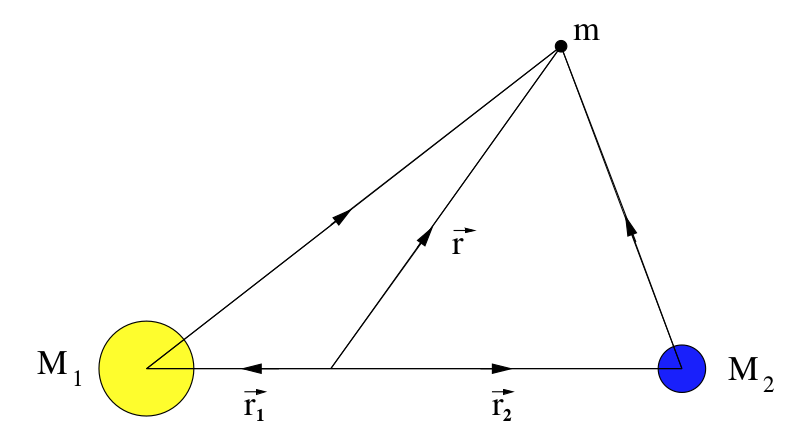
\includegraphics[scale = 0.5]{3_corpos.png}
\caption{Problema restrito de 3 corpos.}
\end{figure}


Temos que as forças atuantes sobre ele são:

\begin{align}
\mathbf{F_1} = -\frac{Gm_1m}{|\mathbf{r}-\mathbf{r_1}|^3}(\mathbf{r}-\mathbf{r_1}) && \mathbf{F_2} = -\frac{Gm_2m}{|\mathbf{r}-\mathbf{r_2}|^3}(\mathbf{r}-\mathbf{r_2})
\end{align}

Nessas condições, chamamos de pontos de Lagrange os pontos que permitem uma órbita estacionária para o terceiro corpo, mantendo constantes as distâncias entre os três corpos.

Como $\mathbf{r_1}$ e $\mathbf{r_2}$ são funções do tempo, torna-se mais conveniente tratar do problema num referencial baricêntrico que gira com velocidade angular constante $\omega$. Nesse caso, devemos levar em consideração as forças de inércia:

\begin{equation}
\mathbf{F_{IN}} = -m\mathbf{\omega} \times (\mathbf{\omega} \times \mathbf{r}) -2m(\mathbf{\omega} \times \mathbf{\dot{r}}) 
\end{equation}

Onde o primeiro termo corresponde à força centrífuga e o segundo, à força de Coriolis. Note que nesse referencial, os pontos de Lagrange correspondem a pontos de equilíbrio estático, nos quais a força resultante (incluindo as forças de inércia) é nula. Para uma solução estática, devemos, é claro, ter que $\mathbf{\dot{r}}=0$. Escolhendo coordenadas cartesianas convenientemente alinhadas, temos:

\begin{eqnarray}
\boldsymbol{\omega} & = & \omega\mathbf{\hat{k}} \\
\mathbf{r} \; & = & x\mathbf{\hat{i}} + y\mathbf{\hat{j}} \\
\mathbf{r_1} & = & -\alpha R\mathbf{\hat{i}} \\
\mathbf{r_2} & = & \beta R\mathbf{\hat{i}} \\
\end{eqnarray}

Onde,

\begin{align}
\alpha = \frac{-m_2}{m_1+m_2} && \beta = \frac{m_1}{m_1+m_2}
\end{align}

Escrevemos então a força resultante sobre o terceiro corpo:

\begin{eqnarray}
\mathbf{F_R} = & \mathbf{F_{IN}} + \mathbf{F_1} + \mathbf{F_2} & = 0 \\
= & m\left[\omega^2\mathbf{r} -G(m_1+m_2)\left(\frac{\beta(\mathbf{r}-\mathbf{r_1})}{|\mathbf{r}-\mathbf{r_1}|^3} + \frac{\alpha(\mathbf{r}-\mathbf{r_2})}{|\mathbf{r}-\mathbf{r_2}|^3}\right) \right] & = 0 \\
= & m\omega^2 \left[\left(x - \frac{\beta(x+\alpha R) R^3)}{((x+\alpha R)^2 + y^2)^{3/2}} - \frac{\alpha(x-\beta R) R^3)}{((x-\beta R)^2 + y^2)^{3/2}}\right)\mathbf{\hat{i}} + \left(y - \frac{y R^3}{((x+\alpha R)^2 + y^2)^{3/2}} - \frac{y R^3}{((x-\beta R)^2 + y^2)^{3/2}}\right)\mathbf{\hat{j}}\right] & =0
\end{eqnarray}

E queremos os pares ordenados (x,y) onde a força se anula. Vemos que não é trivial resolver esse sistema diretamente. Entretanto, podemos induzir as respostas levando em consideração suas simetrias.

Considerando a simetria por reflexão no eixo x, temos que a função tem que se anular na reta $y=0$. Definimos:

\begin{equation}
x \equiv (u+\beta)R
\end{equation}

De maneira que u mede a distância do corpo até $m_2$ em unidades de R. A equação resulta em:

\begin{eqnarray}
R(u+\beta) - \frac{\beta R^4(u+\beta+\alpha)}{R^3(u+\beta+\alpha)^3}- \frac{\alpha R^4u}{R^3u} & = & 0 \\
R\left[\frac{u^2(u+\beta+\alpha)^2(u+\beta)-\beta u^2 - \alpha(u+\beta+\alpha)^2}{u^2(u+\beta+\alpha)^2}\right] & = & 0 \label{poliu}
\end{eqnarray}

E o problema se passa a ser encontrar as raízes do polinômio de grau 5 no numerador da (\ref{poliu}), onde não há uma solução fechada. Nesse caso, consideraremos a hipótese $\alpha << 1$ e faremos uma aproximação de primeira ordem.

\section{Generalizações}
% TODO Discutir resultados recentes que generalizam a noção de ponto de Lagrange.
% http://iopscience.iop.org/article/10.1086/513736/meta
% http://iopscience.iop.org/article/10.1086/423214/meta

O estudo de pontos análogos ao de Lagrange para sistemas de três corpos continua até hoje. O objetivo dessa seção é apresentar qualitativamente resultados recentes relacionados em forma ou conteúdo à teoria abordada.

No estudo de sistemas binários de estrelas, um dos modelos fundamentais da estrela é o de Roche. Nele, modela-se a estrela hidrodinamicamente como um ponto contendo toda a sua massa cercado por um envelope de massa nula, traçando, portanto, . O potencial generalizado é expresso, para uma das estrelas, num referencial baricêntrico rotacionando uniformemente com eixo $x$ no sentido que une os centros das duas estrelas, por

\begin{equation}
    U_{eff, 1} = -\frac{Gm_1}{||\mathbf{r}_1||}-\frac{Gm_2}{||\mathbf{r}_2||}-\frac{1}{2}\omega^2(x^2 + y^2)+\frac{Gm_2x}{||\mathbf{r}_1 - \mathbf{r}_2||^2},
\end{equation}

incluindo, agora, no último termo, efeitos de maré devido à companheira. A equação de movimento para um elemento da estrela, nessa situação, é

\begin{equation}
    \label{eq:rochemotion}
    \ddot{\mathbf{r}}_1 = -\frac{1}{\rho}\nabla P - \nabla U_eff - 2\mathbf{\omega}\times\dot{\mathbf{r}}_1
\end{equation}

onde $\rho$, a densidade volumar de massa da estrela, e $P$, a pressão do material na estrela, descrevem a hidrodinâmica do material estelar devido à rotação do corpo. Caso o movimento orbital e a rotação da estrela sejam sincrônicos, não há movimento do elemento de massa no nosso referencial, reduzindo a \ref{eq:rochemotion} ao equilíbrio hidrostático

\begin{equation}
    \frac{1}{\rho}\nabla P = -\nabla U_{eff, 1},
\end{equation}

donde se conclui que a densidade e pressão, e portanto os formatos possíveis da estrela, dependem unicamente do potencial, sendo dados pelas curvas equipotenciais.

Essa situação, que é o caso estático do binário de estrelas, admite, para órbitas não ecêntricas, pontos de Lagrange essencialmente idênticos aos já descritos.

% TODO Discussão do lóbulo de Roche talvez?